% Provides macros manipulating strings of tokens.
\RequirePackage{xstring}
% Store the jobname as a string with category 11 characters.
\edef\normaljobname{\expandafter\scantokens\expandafter{\jobname\noexpand}}
\StrBehind{\normaljobname}{exer-}[\exercisenumber]

\documentclass[
  coursecode={CMPE 251},
  assignmentname={Exercise \exercisenumber},
  studentnumber=20053722,
  name={Bryan Hoang}
]{
  ltxanswer%
}

\marksnotpoints{}

\usepackage{bch-style}

\begin{document}
  \begin{questions}
    \question[2]{}
    This week we will experiment with the k-Nearest-Neighbour predictor. It has two basic parameters: how many neighbours to consider (i.e., the k), and whether or not close neighbours should have greater influence on the prediction result.

    Try to classify the type of wine varying these parameters to see how well you can do.
    \begin{solution}
      \begin{answerfigure}
        \begin{answerfigure}
          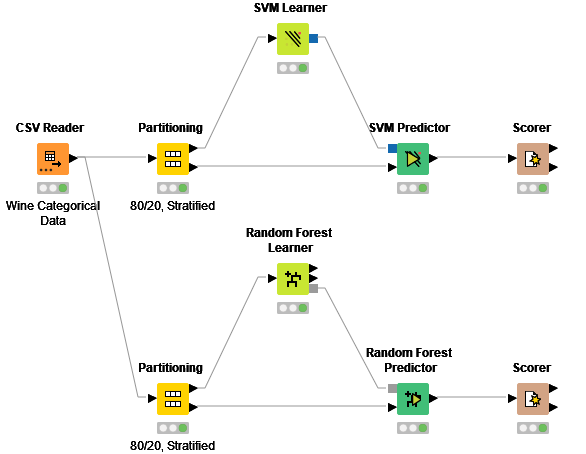
\includegraphics[width=0.75\textwidth]{wine-workflow.png}
          \captionof{figure}{KNIME workflow used}\label{fig:wine-workflow}
        \end{answerfigure}
        \begin{answerfigure}
          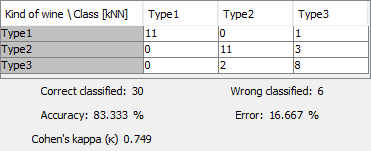
\includegraphics[width=0.75\textwidth]{wine-7nn-confusion-matrix.png}
          \captionof{figure}{Confusion matrix of "7nn" predictor}\label{fig:wine-7nn-confusion-matrix}
        \end{answerfigure}
      \end{answerfigure}
    \end{solution}

    \question[2]{}
    This technique also allows you to output the probabilities associated with each prediction. Have a look at these and see whether most predictions are clear cut, or whether some are quite difficult.
    \begin{solution}
      \begin{answerfigure}
        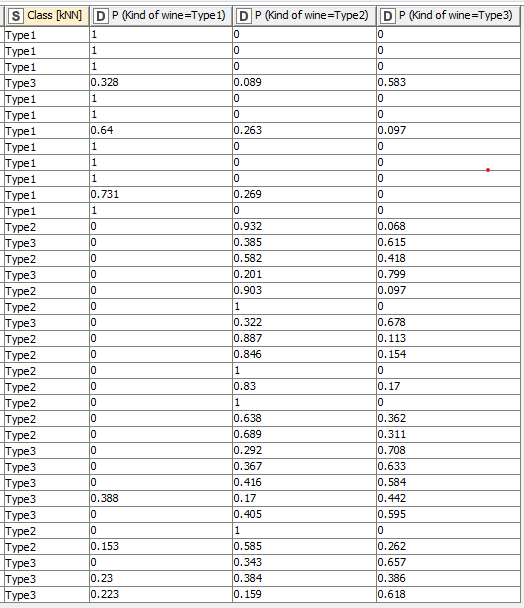
\includegraphics[width=0.75\textwidth]{wine-7nn-class-probabilities.png}
        \captionof{figure}{Class probabilities of "7nn" predictor}\label{fig:wine-7nn-class-probabilities}
      \end{answerfigure}
    \end{solution}
  \end{questions}
\end{document}
